\section{Study 1: Model Building}
The appeal of real world scenario is transfer of results. But such experiments suffer from lack of repeatability and reproducibility because of the large number of variables involved. Repeating a route, introduces learnable landmarks that change performance.  Events of interest happen unpredictably and infrequently. Establishing ground truth in such cases is also non-trivial and sometimes requires manual effort like scoring or annotating video recordings, etc. Experiments in the lab can circumvent a lot of these shortcomings by abstracting out the problem. A common practice in psychophysiology, however, is to have a control condition, followed by a test condition, with a rest period in between. As a consequence, the temporal aspects of psychophysiological signals as they fluctuate, is lost. 

% by allowing researchers to abstract out the problem and focus only on the particular aspects of it that are of interest to them

In collecting this dataset, we wanted the advantage of the lab setting, while still grappling with some of the complexity of real world data. In particular, we wanted to capture the temporal aspects of fluctuating psychophysiological signals while a participant is intermittently multitasking. We settled on an driving like primary task scenario. Attending and responding to notifications is a  secondary task. These two tasks allow investigation of the impact that the timing and modality of the notification would have on the load experienced by the user. 

Our goals with this dataset are to:
\begin{itemize}
\item Experiment with building models that can rapidly track cognitive load in a multitasking driving scenario
\item Study the impact that the timing and modality of an intermittent secondary task has on cognitive load
\end{itemize}

A user study using a driving simulator varied task load,  timing (mediated vs. non-mediated) and modality (audio vs. visual) of notifications being sent to the driver, while they performed the primary sensory motor steering and reaction tasks. The study was setup so that the driving task would randomly switch between low and high workloads. In the mediated condition, the audio notifications would be sent only during the low driving workload condition, in contrast to their random delivery in the non-mediated condition. With regards to modality, audio notifications were delivered via speakers, and visual notifications through Google Glass (Glass). Glass's optics projects the screen at a working distance of 3.5 m, approximately \SI{35}{\degree} elevated from the primary position of the eye. The audio notifications were created using Apple's text-to-speech engine on OS X Yosemite (Speaking voice: Alex; Speaking rate: Normal).



\subsection{Design}
The study was designed as a 2 (Audio/Visual modes) X 2 (Mediated/Non-mediated conditions) repeated measures within subjects study. To control for possible effects of order the study was double counterbalanced for the ?? mode and condition ??factors. Additionally, there was a baseline for each of low and high driving workload conditions. 

\subsection{Participants}
20 people (10 male, 10 female) participated in our study, recruited through a call sent out to students selected randomly from a graduate school population. The mean age of the participants was 26.4 years, with a standard deviation of 2.7 years. Participants were rewarded with a \$40 gift cards for completing the study.

\subsection{Tasks}
A multitasking scenario using a modified driving simulator created a random sequence of high and low workload periods. We elaborate below on the design of the primary driving task, and the secondary notification task.

\begin{figure}
\centering
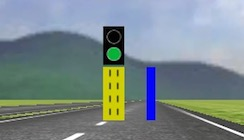
\includegraphics[scale=.8]{sim}
\caption{Screenshot of the ConTRe Task that displays the yellow reference cylinder with the traffic light on top, and the blue tracking cylinder.}
\label{fig:my_label}
\end{figure}

\subsubsection{Primary Task: Driving}
The primary driving task was implemented as the validated  of ConTRe (Continous Tracking and Reaction), which comes as an add-on for OpenDS, an open-source driving simulator~\cite{mahr2012}.  In ConTRe, the driver's task is comprised of steering and reactions to signals that mimic normal driving: operating the brake and acceleration pedals, and using the steering wheel. It differs from normal driving in terms of system feedback. Here the car moves autonomously with a constant speed on a unidirectional straight road consisting of two lanes. Operating the pedals or steering wheel has no effect on changing the speed or direction of the vehicle. Instead, these controls are used to manipulate a laterally moving cylinder, which is rendered in front of the car. 

The simulator shows two cylinders at a constant distance in front of the car: a yellow reference cylinder, and a blue tracking cylinder. The yellow reference cylinder moves autonomously according to an algorithm whose parameters can be set programmatically. The lateral position of the blue tracking cylinder is controlled by the driver through the use of the steering wheel. The cylinder moves left or right depending on the direction and angular velocity of the steering wheel, i.e the steering wheel controls the cylinder's lateral acceleration. The Subject's goal is to track the yellow reference cylinder, by overlapping it with the user-controlled blue cylinder, as closely as possible. This roughly mimics a steering task where the user has to follow a curvy road. A green light below and a red light above mimic a streetlight reaction task  placed on top of the yellow reference cylinder. At any time, neither of the lights or only one is turned on. The red light requires that the driver respond by depressing the brake pedal, while the green light corresponds to the accelerator pedal. As soon as the user reacts to the light by depressing the right pedal, the light turns off.

For the low and high driving workload, the lateral speed of the reference cylinder was set to values that were empirically determined to cause significant differences in driving performance measures. In the experimental conditions, the lateral speed of the reference cylinder was set to psuedorandomly shift between the low and high workload settings. For every shift, the duration of each workload was randomly set by the algorithm, and was programmed to be within specified intervals. 

\subsubsection{Secondary Task: Notifications}
The notification task was based on widely used measures of working memory capacity, which include operation span and reading span tasks~\cite{conway2005}. Working memory has been purported to be involved in a wide range of complex cognitive behaviors, such as comprehension, reasoning, and problem solving as it is thought to reflect primarily domain-general, executive attention demands of the task~\cite{engle2002}. In this work we do not aim to measure working memory per se, but instead want to measure the effect of engaging in a complex cognitive secondary task. Thus, we modify the span tasks for our purposes as described below.

In each condition, Subjects were presented with a series of twenty items, which included ten equations and ten sentences (see Table~\ref{table:span}). The math and sentence notifications were randomly interspersed, so as to prevent the driver from getting into a rhythm of expecting either one. After the driver had read or listened to each item, they indicated its veracity by verbally responding \textit{true} or \textit{false}. Sentences are `true' when they are sensically valid. 

After each item, the subject was presented with an isolated letter. After two, three or four items, the driving task was paused, and they were asked to recall the letters in sequence. This was done to mimic the behavior of drivers who usually attend to notifications while driving, and respond to them, or perform other tasks that require more attention, when stopped at a light, or while driving down a road with no noticeable gradient or curve at a constant speed~\cite{kim2015}. 

\renewcommand{\arraystretch}{1.3}
\begin{table} \centering
\begin{tabular}{@{}ll@{}}\toprule
\textbf{Type} & \textbf{Notification} \\ \midrule 
Math & $2/2 + 1 = 1$ \\ 
Sentence & \multirow{2}{5cm}{After yelling at the game, I knew I would have a tall voice}  \\ & \\
% & \\
\bottomrule
\end{tabular}
\caption{Examples of the two types of notifications }
\label{table:span}
\end{table}


% \subsubsection{Mediation}
% In this work, mediation was primarily involved with the timing of the notifications. In the non-mediated condition, the notification would be displayed on the Glass, or played over speakers at random intervals. In the mediated condition, the bounded deferral technique~\cite{horwitz2005} was used, where the notifications would be delayed while the driver was in a high workload setting. The notification would then be delivered a few seconds into the low workload setting. Mediation timing was chosen by an experimentor   could determine when to deliver the intervention message. If it was the case that a notification had been delivered, and the workload setting changed from low to high before the driver responded, there were different options depending on the modality. For the audio mode, the notification could be paused and continued at the next low workload period, or simply repeated. In the visual mode, the notification could be hidden till the next low workload period, when it would become visible again. The overall goal was not to overload the driver. The experimentor was tasked with using their intuition and judgement to avail of the different options, given the situation.

% Before each condition, participants were told which mode of notification they would be receiving, i.e.\ audio or visual. However, they did not receive any indication as to whether the notifications would be mediated or not. This was to test whether they would notice the shift in timing.

\subsection{Apparatus}
The Robot Operating System (ROS Hydro) was used to synchronize signals from the different components of the experimental setup. This included the simulator, physiological sensors, and the audio-visual feeds, all of which were running on different machines. Each component publishes messages via ROS Nodes to the server, which records the data as rosbags and writes it to disk. A Logitech camera along with mic and audio mixer was used to capture audio-visual information. Participants controlled the simulator using a Logitech G27 Racing Wheel.

\subsection{Physiological Sensors}
Physiological signals were captured and recorded using the Biopac's BioNomadix monitoring devices for ECG, Photoplethysmograph (PPG), EMG, Respiration, Skin Temperature, Electrodermal activity (EDA), and Impedance Cardiography (ICG). Pupil dilation and eye gaze was captured using Pupil Pro hardware\footnote{http://pupil-labs.com/pupil/}, which is a head mounted mobile eye tracking platform.

Since the hands of the participant were occupied for driving, we placed the PPG and EDA sensors on the participant's left toe \& instep, respectively~\cite{vanDooren2012}. The Facial EMG sensor was placed just above their left eyebrow to measure activation of the corrugator supercilii muscle, which is associated with frowning. Two skin temperature sensors were placed on the tip of the nose and on the left cheek. The ECG, impedance cardiography and respiration sensors were placed in the default positions, i.e. on the chest and neck. 

\subsection{Methodology}
Participants  were guided through an informed consent process, followed by an overview of the study. They were aided through the process of having a number of sensors attached to their body for the purposes of recording their physiological responses. The participant was then seated in the simulator and shown how notifications would be delivered on the Glass, and through binoral speakers. 

The dataset collection was split in two parts: baseline \& experimental. The baseline section records physiological measures for low and high driving workload separately. The experimental section records physiological measures for the multitasking scenario described in Section 3.3.  

\subsubsection{Baseline}
Each participant was taken through a series of practice runs to get them comfortable with the primary driving task. When done with the practice, the low benchmark was recorded using the low workload setting on the simulator. After a minute, they were asked to repeat a series of ten sentences that were read out to them, one-by-one, while they were still stearing and reacting to lights in the simulator. The same routine was performed to record the high benchmark using the high workload setting on the simulator. 

\subsubsection{Experimental}
This was followed by another set of practice rounds that combined both the driving task (with the randomly alternating workloads) and the notifications task. The notification task included a set of five items, three of which were equations, with the rest being sentences. This provided the participants with a sense of what to expect during the actual trials. The practice trials could be repeated if necessary. The participants then moved on to the experimental trials. Each participant had a total of four trials, one for each condition. The entire study lasted approximately 2 hours.




